% Created 2015-12-13 Sun 11:26
\documentclass[graduation-thesis]{mlarticle}
     \usepackage[dvipdfmx]{graphicx}
     \usepackage{url}
     \usepackage{atbegshi}
     \AtBeginShipoutFirst{\special{pdf:tounicode EUC-UCS2}}
     \usepackage[dvipdfmx,setpagesize=false]{hyperref}
          \usepackage[dvipdfmx]{color}
\usepackage{url}
\usepackage{float}
\usepackage[setpagesize=false]{hyperref}
\usepackage{ascmac}
\usepackage{here}
\usepackage{txfonts}
\usepackage{listings, jlisting}
\author{61200185 情報工学科 縣直道}
\date{\today}
\title{}
\begin{document}


\makeatletter
\renewcommand{\thetable}{
        \thesection.\arabic{table}
} %「表(章番号)-#.」と表記するための措置
\@addtoreset{table}{section}
  
\renewcommand{\thefigure}{
        \thesection.\arabic{figure}
}
\@addtoreset{figure}{section} %「図(章番号)-#.」と表記するための措置

\setcounter{page}{1}

\pagenumbering{roman}
\tableofcontents
\clearpage

\pagenumbering{arabic}

\definecolor{keywords}{RGB}{255,0,90}
\definecolor{comments}{RGB}{0,0,113}
\definecolor{red}{RGB}{160,0,0}
\definecolor{green}{RGB}{0,150,0}
 
\lstset{
        basicstyle=\ttfamily\footnotesize, 
        frame=single,
        keywordstyle=\color{keywords},
        commentstyle=\color{comments},
        stringstyle=\color{red},
        showstringspaces=false,
        identifierstyle=\color{green},
        }

\section{はじめに}
\label{intro}

\subsection {背景}
\label {intro:background}
現在,仮想化技術が普及してきており,様々なサービスの基盤技術として広く用いられている.
仮想化技術の利用例として,クラウドコンピューティングやInfrastructure as a Service (IaaS) が挙げられる.
クラウドコンピューティングでは,データセンタに配置されている大量の物理マシンを,多くの利用者が同時に利用する.
物理マシンという限られたリソースを仮想化することで,複数の利用者が安全にリソースを共有することが可能になり,利用者には柔軟なハードウェア資源の構成を提供することができる.
IaaS は仮想化されたコンピュータ基盤をインターネット経由でサービスとして提供するものである.
クラウドコンピューティングを利用することで,高い可用性を得ることができ,大規模な並列計算なども行いやすくなる.

クラウド環境上では,一台の仮想マシン上で,一つのアプリケーションのみを実行する場合がほとんどである.
これは,クラウド環境上では,物理マシンというリソースを増やすことなく仮想マシンを増やすことが可能であり,複数のアプリケーションを実行する場合には仮想マシンを増やすことで対処可能なためである.
ある利用者が複数のアプリケーションを実行したいと考えた場合,一つの仮想マシン内で実行するのではなく,それぞれのアプリケーションに対して仮想マシンを割り当てる.
このようにすることで,それぞれのアプリケーションが互いのパフォーマンスに影響することなく動作する.

また,このようなクラウド環境上の仮想マシンには,ほとんどの場合,物理マシン上で利用されるような汎用オペレーティングシステム(Linux,Windows,*BSD)が利用される.

\subsection {問題点}
\label {intro:problem}
汎用オペレーティングシステムは,高度な抽象化,機能を多数備えている.
オペレーティングシステム上で動作するアプリケーションが固定されている場合,それらの抽象化,機能は不要となる.

クラウド環境上の仮想マシンでは,ほとんどの場合,動作するアプリケーションが固定されている.
仮想マシンに汎用オペレーティングシステムを利用する場合,使用されることのないオペレーティングシステムの機能のために,カーネルイメージのサイズが増大し,セキュリティにも問題を抱えることになる. 
カーネルイメージのサイズが大きいと仮想マシンのサイズも大きくなり,仮想マシンの起動時間も大きくなる.
クラウド環境では,一つのアプリケーションごとに一台の仮想マシンを立ち上げるため,これらは大きな問題となる.

この問題の解決案として,あるアプリケーションに特化したオペレーティングシステムを開発するという方法が考えられる.
しかし,オペレーティングシステムの開発は難しく,誤った実装が行われた場合システム全体に影響を及ぼしてしまう.
さらに,アプリケーションごとに新たにオペレーティングシステムを開発する必要があるという問題もある.
したがって,アプリケーションごとに特化したオペレーティングシステムを開発するという手法は,現実的とは言えない.


\subsection {提案}
\label{intro:proposal}
本研究では,汎用オペレーティングシステムから,アプリケーションが必要としない機能を自動的に削除することで,アプリケーションに特化したカーネルを生成する.
アプリケーションのソースコードを静的解析することで,必要となるオペレーティングシステムの機能を絞り込み,ブートに必要な部分と絞り込んだ機能を実装している部分のみを残すよう,カーネルのソースコードを書き換える.
自動的にカーネルを改変することで,アプリケーションごとに特化したオペレーティングシステムを開発する必要があるという問題点を解決する.

\subsection {実装}
\label{intro:implementation}
% TODO: gcov と openstack のリファレンス
まず,Linux カーネルソースコードの内,ブートに必要な部分とそうでない部分を分類する必要がある.
アプリケーションが使用する機能以外のすべてのソースコードを削除してしまうとブートすることが出来ないオペレーティングシステムになってしまう.
本研究では,この分類を行う手法を実装した.

本研究では,ブートに必要な部分を判別するため,\texttt{gcov} を用い,ブートまでのコードカバレッジを取得した.
ここから,ブートまでに一度も実行されていなかった関数を判別することができる.

ブートまでに一度も実行されていなかった関数をすべて削除したカーネルはブートすることが出来なかったため,Open Stack 上でカーネルがブートすることをテストできる環境を構築し,現在実験中である.

\subsection {論文の構成}
\label{intro:arch}
本論文の構成をいかに示す.
第\ref{relative}章では,本研究と関連する研究を紹介する.
第\ref{proposal}章では,本研究が提案する手法について説明する.


\clearpage
\section{Infrastructure as a Service}
Infrastructure as a Service(IaaS)とは,クラウドコンピューティングの一種で,ネットワークを経由して,CPU,ストレージ,OS,ミドルウェアなどの基盤を提供するサービスのことである.
IaaSでは,仮想化技術が応用されており,ハードウェア資源を仮想化して利用者に提供することで,その物理的構成に依らない柔軟で効率的な活用を達成している.
ハードウェア資源の構成を変更することは,通常であれば物理的構成を変更する必要があり,ネットワークを経由して基盤を利用するIaaSの場合,物理的構成を変更することは難しい.
仮想化技術を用いることで,ハードウェア資源の構成を,物理的構成と切り離して変更することが可能にない,ネットワークを経由してハードウェア資源の構成を変更することが容易になる.
IaaSの最大の特徴は,ハードウェア資源の構成を柔軟に変更できる点にある.

IaaSは,Webアプリケーションサーバや大規模な並列計算など,様々な用途に利用することができる.
IaaSの利用者は,ネットワークを経由していることを意識することなく,その基盤上でアプリケーションを実行することができる.
WebアプリケーションサーバとしてIaaSを利用する場合,Webアプリケーションへのアクセスの急増に合わせて,ハードウェア資源の増強を,容易に行えるといった利点がある.
また,大規模な並列計算のような,計算資源を大量に必要とするアプリケーションの場合,IaaSを利用することで,計算資源を確保しやすくなる.

このような仮想化環境を利用したアプリケーションの実行が,近年普及してきている.

通常,IaaSの利用者は,IaaSが提供するハードウェア資源上で,汎用オペレーティングシステムを利用する.
一方,IaaS環境上でアプリケーションを実行する際には,一つのアプリケーションに対して一台の仮想マシンを割り当てる場合が多い.
これは,IaaSを利用する場合,仮想マシンを増やすことが非常に容易であるためである.
このような運用をすることで,複数のアプリケーションがそれぞれ互いに影響することなく実行される.
一台の仮想マシン内で,一つのアプリケーションのみを実行する場合,汎用オペレーティングシステムの提供する機能の多くは不要になる.
汎用オペレーティングシステムは非常に多くの機能を提供しているためである.
例えば,実行するアプリケーションが一つのプロセスである場合,プロセスを新しく生成するforkの機能は不要である.
この場合,利用するカーネルのサイズが,不要な機能のために増大し,メモリを無駄に使用することになってしまう.
カーネルから不要な機能を削除できれば,カーネルのサイズを小さくすることができ,メモリ使用量の削減,セキュリティの向上につながる.

\clearpage
\section {関連研究}
\label{relative}

本章では,本研究と関連する研究を紹介する.
Exokernel は,極小さなカーネルに,ライブラリとして高度な機能を付加する構成を提案している.
OSv は,仮想マシン上で一つのアプリケーションのみを実行する環境に特化したオペレーティングシステムを開発した.
Unikernel は,カーネルコンパイル時に,オペレーティングシステムの機能の有無を設定することができるカーネルである.

\subsection {Exokernel: An Operating System Architecture for Application-Level Resource Management}
\label{relarive:exokernel}
カーネルのサイズを小さくするために,極単純な機能のみを持つカーネルに,Library OS として高レベルな抽象化などの機能を付加するという構成を提案している.

中心となる極小さなカーネルは,ハードウェア資源にアクセスするための低レベルなインターフェースを提供する役割のみを持つ.
プロセス,ファイル,アドレス空間,プロセス間通信といった高レベルな抽象化は,カーネルの提供するインターフェースを用いて,すべてカーネル外のライブラリとして実装される.
このような構成にすることで,アプリケーションが必要とする抽象化のみを提供することができ,アプリケーションが直接ハードウェア資源にアクセスすることも可能となる.
また,アプリケーションが必要とする機能のみをもつオペレーティングシステムを構築できるため,オペレーティングシステムによるオーバヘッドやメモリ使用量の増加といった問題を解決することができる.

% TODO: Exokernel の本研究との関連をうまく説明

Exokernel の構成では,アプリケーションを変えると,そのアプリケーションが必要とする抽象化を選択し再構成する必要が生じる.

\subsection {OSv - Optimizing the Operating System for Virtual Machines}
\label{relative:unikernel}
OSv は,一つのアプリケーションをクラウド環境上で実行することに特化したオペレーティングシステムである.

標準的な仮想マシンの構成を図\ref{fig:vm}に示す.

\begin{figure}[H]
  \begin{center}
    \includegraphics[width=8.0cm]{images/vm.png}
    \caption{仮想マシンの構成}
    \label{fig:vm}
  \end{center}
\end{figure}

仮想マシンでは,ハードウェアをハイパーバイザが仮想化し,ハイパーバイザ上でオペレーティングシステムが動作する.

仮想マシン上で一つのアプリケーションのみを実行する場合,オペレーティングシステムが持つハードウェア抽象化やプロセス間Isolationといった役割は,ハイパーバイザが担っており,不要な抽象化が重なりオーバヘッドになる.

\ref{intro:background}で述べたように,クラウド環境上の仮想マシンでは,一つのアプリケーションのみを実行する場合がほとんどである.
仮想マシン上で一つのアプリケーションのみを実行するという環境では,
アプリケーションにバグがあったり,悪意あるアプリケーションが動作した場合であっても,
仮想マシン上ではそのアプリケーションしか実行されておらず,同じ物理マシン上で動作する他の仮想マシンは,ハイパーバイザによって保護されているため影響を受けない.

OSvは,仮想マシン上で一つのアプリケーションのみを実行することを前提にし,ハードウェア抽象化やプロセス間Isolationの機能をオペレーティングシステムから削除した.
また,Posix API互換のAPIと独自のAPIを提供している.Posix API互換のAPIでは,システムコールは単なる関数呼び出しに過ぎず,Linuxなどにおけるシステムコールが必要とする,ユーザモードから特権モードへの切り替えや引数のコピーなどは行われない.
このようにすることで,Linux上で動作していたネットワークインテンシブなアプリケーションについて,25%のスループット向上,47%のレイテンシ削減を,アプリケーションを改変することなく実現した.
また,OSv独自のネットワークAPIを使用するようアプリケーションの改変を行い,スループットが290%向上した.

OSvは,仮想マシン上で一つのアプリケーションのみを実行する環境に特化したオペレーティングシステムを開発したが,
実行するアプリケーションに特化したオペレーティングシステムを提供する手法ではない.
また,その前提上,forkやexecといった関数は提供されていないため,これらを用いるアプリケーションを実行することが出来ない.


\subsection {Unikernel: Library Operating Systems for the Cloud}
\label{relative:unikernel}
Unikernelは,コンパイル時に,オペレーティングシステムが提供する機能の有効,無効を設定することができるカーネルを提案した.
OSvと同様に,仮想マシン上で一つのアプリケーションのみを実行する環境を想定し,
そのアプリケーションが必要としないオペレーティングシステムの機能を無効にしてコンパイルすることで,
カーネルのサイズを縮小し,無駄なコードを削減した.

% TODO: library os で一つのサブセクションにして,その中でUnikernelとExokernelを紹介する?OSvもLibrary OSなのでまとめるべき?
% TODO: Dune や Arrakis はどうやって紹介するか

OSvやUnikernelは仮想マシン上で一つのプロセスのみを実行するという環境を想定しており,HTTPサーバのように一つのアプリケーションがforkして複数のプロセスをもつというようなものは実行できない.
このような場合,OSvやUnikernelでは,もう一台仮想マシンを起動し,VM間通信を行う必要がある.


\clearpage
\section{提案}
\label{proposal}

\subsection{概要}
\label{proposal:abstruction}
本研究では,クラウド環境を想定し,あるアプリケーションのみを実行することに特化したオペレーティングシステムになるよう,汎用オペレーティングシステムを自動的に改変することでカーネルを軽量化する手法を提案する.
アプリケーションを実行するためには,アプリケーションが利用する機能を実装する部分と,ブートに利用される部分が必要となる.
そこで,図\ref{fig:kernelcode}で網掛けになっている部分を削除するよう,Linuxカーネルのソースコードを改変する.

\begin{figure}[H]
  \begin{center}
    \includegraphics[width=8.0cm]{images/kernelcode.png}
    \caption{Linuxカーネルの改変}
    \label{fig:kernelcode}
  \end{center}
\end{figure}

アプリケーションが変わってもカーネルの自動軽量化が適用できるようにするため,
アプリケーションのソースコードを静的解析し,そのアプリケーションが必要とするオペレーティングシステムの機能を絞り込む.

また,アプリケーションが必要とする機能を実装する部分以外にも,ブートに必要な部分は削除しないようにする必要がある.
そこで,まず,カーネルソースコードを,ブートに必要な部分とそうでない部分に分類する必要がある.

本研究では,関数単位での削除のみを対象とし,Linuxカーネルを改変する.
関数単位の削除とは,必要でないと判断できる関数の定義を,panicのみを呼び出すようソースコードを書き換えることである.

\begin{lstlisting}[language=C, caption=ftruncate関数(改変前), label=code:before]
  SYSCALL_DEFINE2(ftruncate, unsigned int, fd, unsigned long, length)
  {
    return do_sys_truncate(path, length);
  }
\end{lstlisting}
\begin{lstlisting}[language=C, caption=ftruncate関数(改変後), label=code:before]
  SYSCALL_DEFINE2(ftruncate, unsigned int, fd, unsigned long, length)
  {
    #ifdef _LINUX_KERNEL_H
    panic("Execute eliminated function(ftruncate).");
    #endif
  }
\end{lstlisting}

\subsection{静的解析}
\label{proposal:static}
オペレーティングシステムの機能をアプリケーションから利用するには,システムコールを呼び出す必要がある.
つまり,アプリケーションが呼び出しているシステムコールが分かれば,どの機能が必要であるか判別することができる.
そこで,アプリケーションのソースコードを静的解析し,コールグラフを生成する.
アプリケーションのコールグラフから,システムコールの呼び出しを発見する.
アプリケーションが利用しているライブラリについても同様の解析を行い,システムコールの呼び出しを発見する必要がある.

また,カーネルのソースコードも静的解析を行い,コールグラフを生成する.
システムコールとしてアプリケーションに提供されているインターフェースとなる関数が,その内部で呼び出している関数を再帰的に発見する必要がある.
アプリケーションの静的解析によって必要であるとわかったシステムコールが,その内部で必要としている関数も,削除しないようにする必要があるためである.

コールグラフを用いた解析は,関数単位での解析となる.
そのため,カーネルのすべての関数について,必要か不要かを判別することができる.
一方,アプリケーションがシステムコールを発行する際,システムコールに引数として渡す値が固定されているという場合がある.
例えば,開かれたファイルディスクリプタに関する操作を行うfcntlシステムコールのシグネチャはソースコード\ref{fcntlsig}のようになっている.

\begin{lstlisting}[language=C, caption=fcntlシステムコールのシグネチャ, label=fcntlsig]
  int fnctl(int fd, int cmd, ... /* arg */);
\end{lstlisting}

第二引数には26種類のフラグを指定することができる.
fnctlには,指定された値によって,様々な処理を行う.
\texttt{F\_DUPFD}が指定された場合,第一引数で指定されたファイルディスクリプタを複製する.
\texttt{F\_GETFD}が指定された場合,第一引数で指定されたファイルディスクリプタに関連するフラグを読みだす.

fcntlは,引数に渡された値のチェックを行った後,do\_fcntl関数を呼び出す.
ソースコード\ref{fcntlimpl}にdo\_fcntlの実装の一部を抜粋する.

\begin{lstlisting}[language=C, caption=do\_fcntlの実装(抜粋), label=fcntlimpl]
static long do_fcntl(int fd, unsigned int cmd, unsigned long arg,
                struct file *filp)
{
        long err = -EINVAL;

        switch (cmd) {
        case F_DUPFD:
                err = f_dupfd(arg, filp, 0);
                break;
        case F_DUPFD_CLOEXEC:
                err = f_dupfd(arg, filp, O_CLOEXEC);
                break;
        case F_GETFD:
                err = get_close_on_exec(fd) ? FD_CLOEXEC : 0;
                break;
        case F_SETFD:
                err = 0;
                set_close_on_exec(fd, arg & FD_CLOEXEC);
                break;
\end{lstlisting}

fcntlは第二引数の値に応じて関数を呼び出し,処理の本体はその呼び出す関数が行うようになっている.
ここで,アプリケーションにおけるfcntlのすべての呼び出しについて,指定されることがないフラグがあれば,そのフラグを部分は不要になる.

このような最適化を行うためには,アプリケーションコードとカーネルコード,双方について,コントロールフローの解析を行う必要がある.

アプリケーションのコントロールフロー解析は,システムコールに渡す引数の取り得る値を列挙するために行う.
例えば,ソースコード\ref{exapp}のような,ファイルの内容をコピーするだけの単純なアプリケーションについて考える.

\begin{lstlisting}[language=C, caption=アプリケーションの例, label=exapp]
    char buf[1024];
    int from_fd = open(argv[1], O_RDONLY);
    read(from_fd, buf, 1024);
    int open_flg = O_WRONLY;
    if (argc > 2 && strcmp(argv[2], "-c") == 0) {
      open_flg |= O_CREAT;
    }
    int to_fd = open("app.txt", open_flg);
    write(to_fd, buf, 1024);
    close(from_fd);
    close(to_fd);
\end{lstlisting}

このアプリケーションのコントロールフローグラフは,図\ref{fig:controlflow}のようになる.

\begin{figure}[H]
  \begin{center}
    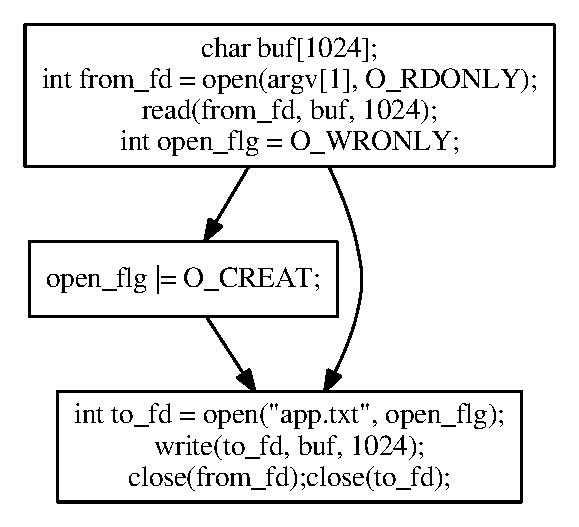
\includegraphics[width=6.0cm]{images/controlflow.eps}
    \caption{アプリケーションのコントロールフローグラフ例}
    \label{fig:controlflow}
  \end{center}
\end{figure}

この時,openシステムコールに渡される第二引数はopen\_flgは,O\_WRONLYかO\_WRONLY $|$ O\_CREAT のどちらかであることがわかる.


カーネルコードのコントロールフロー解析は,アプリケーションの解析で得られたシステムコールにの引数になり得る値についての情報を利用し,switch文中の不要なcase節や不要なif文を識別するために行う.

\subsection{カーネルのブート}
\label{propo:boot}
カーネルのソースコードには,システムコールとしてアプリケーションに提供される関数に関連するコード以外にも,多くの関数が含まれている.
デバイスを認識し初期化するコードや,マウント処理などである.
マシンがブートする際,カーネルはハードウェアやメモリ,ファイルシステムの初期化を行い,initプロセスを起動する.
したがって,アプリケーションが必要とするシステムコールに関連するコード以外のすべてのコードを削除してしまうと,そのカーネルはブートすることができなくなってしまう.

そこで,カーネルを改変する際,ブートに必要な部分を改変しないようにする必要がある.
そのために,カーネルコードの内,ブートに必要な部分とそうでない部分を分類する.

カーネルのソースコードでは \_\_initというマクロが利用されている.
これは,kernel/include/linux/init.hとkernel/include/linux/compiler.hで,ソースコード\ref{code:__init}のように定義されている.

\begin{lstlisting}[language=C, caption=\_\_initマクロの定義, label=code:__init]
  #define __init __section(.init.text) __cold notrace
  #define __section(S) __attribute__ ((__section__(#S)))
\end{lstlisting}

これは,関数を修飾し,その関数が初期化処理用の関数であることを宣言している.
\_\_initで修飾された関数は,.init.textというセクションに配置される.
.init.textセクションは初期化が終了すると廃棄されるメモリ領域である.
すなわち,\_\_initで修飾された関数はすべてブートに必要な関数であると考えられる.

また,Linuxカーネル内のinit/ディレクトリも同様に初期化に必要な処理を担当するソースコードを含んでいるため,これらもブートに必要な関数であると考えられる.

一方,これら以外にも,ファイルシステムの初期化処理など,カーネルがブート時に実行するべきコードは,Linuxカーネルソース内に広く存在している.

そこで,ブートに必要な部分の分類には,カーネルコードのカバレッジを利用する.
マシンを起動し,カーネルがブートするまでのカバレッジを取得し,そのカバレッジ情報から,ブートまでに実行されていることがわかったコードは,ブートに必要であると判断できる.

しかし,カーネルのブートステップは非常に複雑であり,ブートまでのカバレッジ情報から分類した,ブートまでに実行されていることがわかったコードのみを残すよう,カーネルを改変しても,ブートすることが出来なかった.
そこで,本研究では,ブートに必要な関数を分類するために,一関数ずつブートするかどうかをテストする手法を提案する.

\subsection{Linuxカーネル}
\label{propo:linux}

\subsubsection{コンパイル}
\label{propo:linux:compile}
Linuxカーネルのコンパイルは非常に複雑なものになっている.
Linuxカーネルのソースコードには,カーネル本体のためのソースコード以外にも,カーネルイメージの圧縮や,設定ファイルや環境に合わせたコンパイルを行うためのソースコードが含まれている.

例えば,Linuxカーネル内では,アーキテクチャに依存する値や設定ファイルに応じた値,コンパイルする環境に応じた値を使用する必要がある.
単純なアーキテクチャ依存の値は,arch/ディレクトリ以下の,それぞれのアーキテクチャ用のサブディレクトリ内で定義されているため,特殊な処理は不要だが,設定と関連する値などは,コンパイル時に生成しなければならない.
そこで,Linuxカーネルのコンパイルでは,まず設定ファイルを読み込み,設定依存,環境依存の値をマクロで定義するヘッダファイルをinclude/generated/ディレクトリに生成している.
% TODO: 実際の例をファイル名,関数名レベルで上げる.圧縮とgeneratedがわかりやすいはず
また,Linuxカーネルは通常,gzipを用いて圧縮されている.ブート時のセットアップで,解凍されメモリ上に展開される.
ビルドの過程で,コンパイルされたLinuxカーネルを圧縮し,カーネルイメージを生成する.
Linuxカーネルを圧縮・解凍するためのコードも,ソースコード内のlib/zlib\_deflate/,lib/zlib\_inflate/に含まれている.
したがって,アプリケーションが必要としていない,ブート時にも実行されないコードであっても,単純に削除することは出来ない.


それぞれのソースコード内でも特殊な記述がされている場合が多い.
通常,拡張子.cのファイルはC言語ソースコードであり,他のC言語ソースコードからインクルードされるのは,拡張子.hのヘッダファイルである.
しかし,Linuxカーネル内では,C言語ソースコードが他のC言語ソースコードをインクルードしている例がある.
kernel/bounds.cがこれに該当する.
ソースコード\ref{code:bounds}にkernel/bounds.cの内容を示す.

\begin{lstlisting}[language=C, caption=kernel/bounds.c, label=code:bounds]
/*
 * Generate definitions needed by the preprocessor.
 * This code generates raw asm output which is post-processed
 * to extract and format the required data.
 */

#define __GENERATING_BOUNDS_H
/* Include headers that define the enum constants of interest */
#include <linux/page-flags.h>
#include <linux/mmzone.h>
#include <linux/kbuild.h>
#include <linux/log2.h>
#include <linux/spinlock_types.h>

void foo(void)
{
        /* The enum constants to put into include/generated/bounds.h */
        DEFINE(NR_PAGEFLAGS, __NR_PAGEFLAGS);
        DEFINE(MAX_NR_ZONES, __MAX_NR_ZONES);
#ifdef CONFIG_SMP
        DEFINE(NR_CPUS_BITS, ilog2(CONFIG_NR_CPUS));
#endif
        DEFINE(SPINLOCK_SIZE, sizeof(spinlock_t));
        /* End of constants */
}
\end{lstlisting}

このファイル内では,関数fooの本体内で定数マクロを定義している.
本研究で提案する手法は,関数を削除するものであるため,関数内で定義したマクロもすべて削除されてしまう.
kernel/bounds.cが定義する定数は,このファイルをインクルードするファイルで利用されるものであるため,これらのマクロが削除されるとカーネルをコンパイルすることができない.

さらに,インラインアセンブラも多用されている.
Linuxカーネルは,非常に低レベルな処理を行う必要があるため,C言語レベルで表現できない場合がある.
例えば,プロセススケジューラ内で,実行コンテキストを切り替える処理について述べる.
切り替え前のプロセスのメモリ空間を,切り替え先のプロセスのメモリ空間に切り替え,CPUのレジスタの値を退避・復帰させる必要がある.
これを行うためには,CPUのレジスタを書き換える必要があるため,アセンブラでの記述が必要になる.
このような処理を行うために,Linuxカーネルではインラインアセンブラを利用する.
インラインアセンブラを使用しているコードに,インラインアセンブラ内で関数を定義するプログラムを記述している箇所がある.
その一つがarch/x86/kernel/kprobes/core.c内のjprobe\_return関数である.
ソースコード\ref{code:inlineasm}にその定義を示す.

\begin{lstlisting}[language=C, caption=jprobe\_return関数, label=code:inlineasm]
void jprobe_return(void)
{
        struct kprobe_ctlblk *kcb = get_kprobe_ctlblk();

        asm volatile (
#ifdef CONFIG_X86_64
                        "       xchg   %%rbx,%%rsp      \n"
#else
                        "       xchgl   %%ebx,%%esp     \n"
#endif
                        "       int3                    \n"
                        "       .globl jprobe_return_end\n"
                        "       jprobe_return_end:      \n"
                        "       nop                     \n"::"b"
                        (kcb->jprobe_saved_sp):"memory");
}
\end{lstlisting}

インラインアセンブラ内で,jprobe\_return\_endという関数を定義している.
このようなインラインアセンブラ内での関数定義を含む関数を削除してしまうと,リンク時にエラーになってしまう.


\subsubsection{ブート}
\label{propo:linux:boot}

Linuxカーネルのブートは,環境やタイミングによって実行される関数が異なる.
ハードウェアの認識,初期化は,ブートするマシンの利用しているハードウェアに応じて異なる処理になる.

本研究では,カーネルコードカバレッジを用いてブートに必要な部分の識別を行うことを提案しているが,
ブートの極初期の段階では,カバレッジ情報を書き込むファイルシステムのセットアップが終わっておらず,
その段階でしか実行されないコードは正しく分類できないと考えられる.
そのため,ブートに必要となる部分だけを正確に分類することは非常に難しい.


\clearpage
\section{実装}
\label{implementation}
\subsection{概要}
\label{implementation:abstruction}
提案手法を実装するためには,第\ref{proposal}章で述べた通り,まず,Linuxカーネルのソースコードの内,ブートに必要となる部分を識別する必要がある.
本研究では,Linuxカーネルのブートに必要となる部分を識別する方法を実装した.

Linuxカーネルのコードカバレッジを用いて,ブートに不要であると思われる関数名を取得する.
次に,Linuxカーネルのソースコードを構文解析し,ブートに不要であると思われる関数を削除する.

手法1では,コードカバレッジから,ブートに必要であるとわかった関数以外のすべての関数を削除した.
手法2では,コードカバレッジから,ブートに不要であるとわかった関数をすべて削除した.
手法3では,コードカバレッジから,ブートに不要であるとわかった関数を一つずつ削除し,ブート可能なカーネルを生成できるかテストすつ環境を構築した.


\subsection{ブートに必要な部分の識別}
\label{implementation:boot}
ブートに必要な部分を識別するためには,Linuxカーネルのコードカバレッジを利用する.
コードカバレッジとは,ソースコード全体について,どの部分が何度実行された
コードカバレッジとは,プログラムのソースコード全体に対する実行されたコードの割合を示し,通常はソフトウェアのテストがプログラム全体の内,どれだけテストできているかを示す指標として使われる.
コードカバレッジの取得には,gcovを用いる.
gcovとは,GNU CCと合わせて使用する,プログラムのコードカバレッジを取得するツールである.
\texttt{gcc -coverage main.c}のようにコンパイルすると,\texttt{main.gcno}というファイルと実行ファイルが生成される.
生成された実行ファイルを実行すると,\texttt{main.gcda}というファイルが生成され,\texttt{gcov main.c}とコマンドを実行するとプロファイル結果が出力される.
プロファイル結果の例をソースコード\ref{code:gcov}に示す.

\begin{lstlisting}[caption=gcovの実行結果例, label=code:gcov]

\end{lstlisting}

$:$の右側に,対象となるソースコードが,
$:$の左側に,各行が何度実行されたかが示されている.
ソースコード\ref{code:gcov}の例であれば,関数gのif文の分岐の片方が実行されていないことがわかる.

gcovは,Linuxカーネルと組み合わせることが可能で,Linuxカーネルのビルド設定を変更し,gcovを組み込むことで,カーネルコードのカバレッジが取得できる.
本研究では,Linuxマシンをブートさせた直後のコードカバレッジを利用することで,Linuxカーネルコードのどの部分がブートに必要であるかを判定する.
ブート直後のコードカバレッジで,一度も実行されていないコードはブートプロセスにとって不要であると言える.

Linuxカーネルにgcovを組み込むためには,カーネルのビルド設定をソースコード\ref{code:gcovkernel}のように設定する.

\begin{lstlisting}[caption=gcovを組み込むLinuxカーネルの設定, label=code:gcovkernel]
  CONFIG_DEBUG_FS=y
  CONFIG_GCOV_KERNEL=y
  CONFIG_GCOV_PROFILE_ALL=y
\end{lstlisting}

Linuxカーネルのカバレッジを取得するためには,debugfsをマウントする必要がある.
debugfsとは,Linuxカーネルの内部情報をユーザが参照するためのファイルシステムで,\texttt{mount -t debugfs /sys/kernel/debug}コマンドを実行することでマウントできる.
このようにdebugfsをマウントすると,/sys/kernel/debug/gcov/以下にLinuxカーネルのカバレッジ情報とソースコードとの対応をとるためのファイル群が生成される.
また,/sys/kernel/debug/gcov/resetというファイルも生成されており,このファイルに書き込みを行うと,カバレッジ情報をリセットすることができる.

本研究では,gcovのカバレッジ情報から,関数単位での実行回数を取得する.
\texttt{gcov}コマンドのオプションで,\texttt{-f}を指定すると,関数単位でのプロファイル結果が出力される.
ソースコード\ref{code:gcov}で示したプログラムについて,\texttt{gcov -f main.c}を実行した際の出力を,ソースコード\ref{code:gcovfunction}に示す.

\begin{lstlisting}[caption=関数単位でのプロファイル結果, label=code:gcovfunction]
% gcov -f main.c
Function 'f'
Lines executed:100.00% of 1

Function 'g'
Lines executed:75.00% of 4

Function 'h'
Lines executed:0.00% of 1

Function 'main'
Lines executed:100.00% of 3

File 'main.c'
Lines executed:77.78% of 9
main.c:creating 'main.c.gcov'
\end{lstlisting}

ソースコード\ref{code:gcovfunction}が示すように,関数名と,その関数本体の行数に対する実行された行数の割合が表示される.
Linuxカーネル内の,すべてのソースコードに対して,\texttt{gcov -f}コマンドを実行し,出力結果をパースして,実行された割合が0.00%だった関数名をすべて取得する.

\subsection{関数の削除}
gcovを用いて得た,ブートに不要と思われる関数を,Linuxカーネルから削除するために,Linuxカーネルのソースコードを構文解析し,得られた関数の定義されている行と桁を調べる必要がある.
Linuxカーネルの構文解析には,clangの提供するLibToolingを用いる.

clangとは,C言語,C++,Objectibe-C,Objective-C++用のコンパイラフロントエンドである.バックエンドにはLLVMを採用している.
clangは,これらのプログラミング言語で書かれたソースコードを,構文解析し,抽象構文木に変換する.
変換された抽象構文木には,コンパイルの構文解析以降でプログラムの誤りを検知した際のエラー通知のために,ソースコード中の位置情報が含まれている.
clangの提供するLibToolingというライブラリは,clangをベースにしたツールを支援するためのライブラリである.
これを利用することで,clangに構文解析を任せることができ,抽象構文木に変換されたソースコードにアクセスすることができる.

gcovによるプロファイル結果をパースし,ブートに不要と思われる関数を,その関数の定義されているファイル名と合わせて出力する.
ファイル名と関数名から,LibToolingを用いて実装したツールを用いて,ファイル名,関数本体の始点位置,関数本体の終端位置を取得する.


\subsection{手法1}
\label{implementation:1}

\subsection{手法2}
\label{implementation:2}

\subsection{手法3}
\label{implementation:3}



\section{分析結果}
\label{result}



\section{おわりに}

\subsection{結論}
\subsection{今後の課題}

\clearpage
\section{謝辞}
\label{sec-8}
\clearpage

\bibliographystyle{jplain}
\bibliography{ref}
% Emacs 24.5.1 (Org mode 8.2.10)
\end{document}
